\section{Water}
The water is basically a squared plane (built in the same way of the flat terrain).

\begin{figure}[hbt!]
	\centering
	\subfloat[\centering Plane.]{{
\includegraphics[width=6.3cm]{images/Water.png}}}%
	\qquad
	\subfloat[\centering Vertices, indices and faces.]{{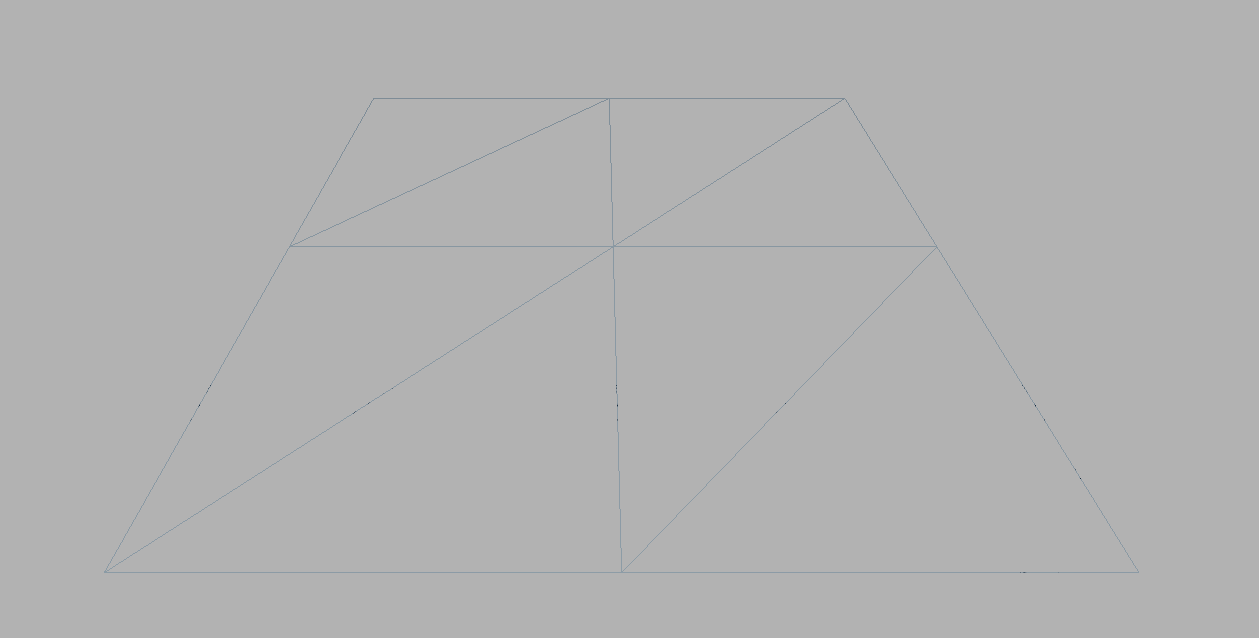
\includegraphics[width=6.3cm]{images/WaterNoVert.png} }}%
	\caption{}
\end{figure}